\documentclass{standalone}
\begin{document}
	\begin{frame}[noframenumbering]{Timing}{Measuring the time performances}
		\begin{columns}
			\begin{column}{.6\textwidth}
				\centering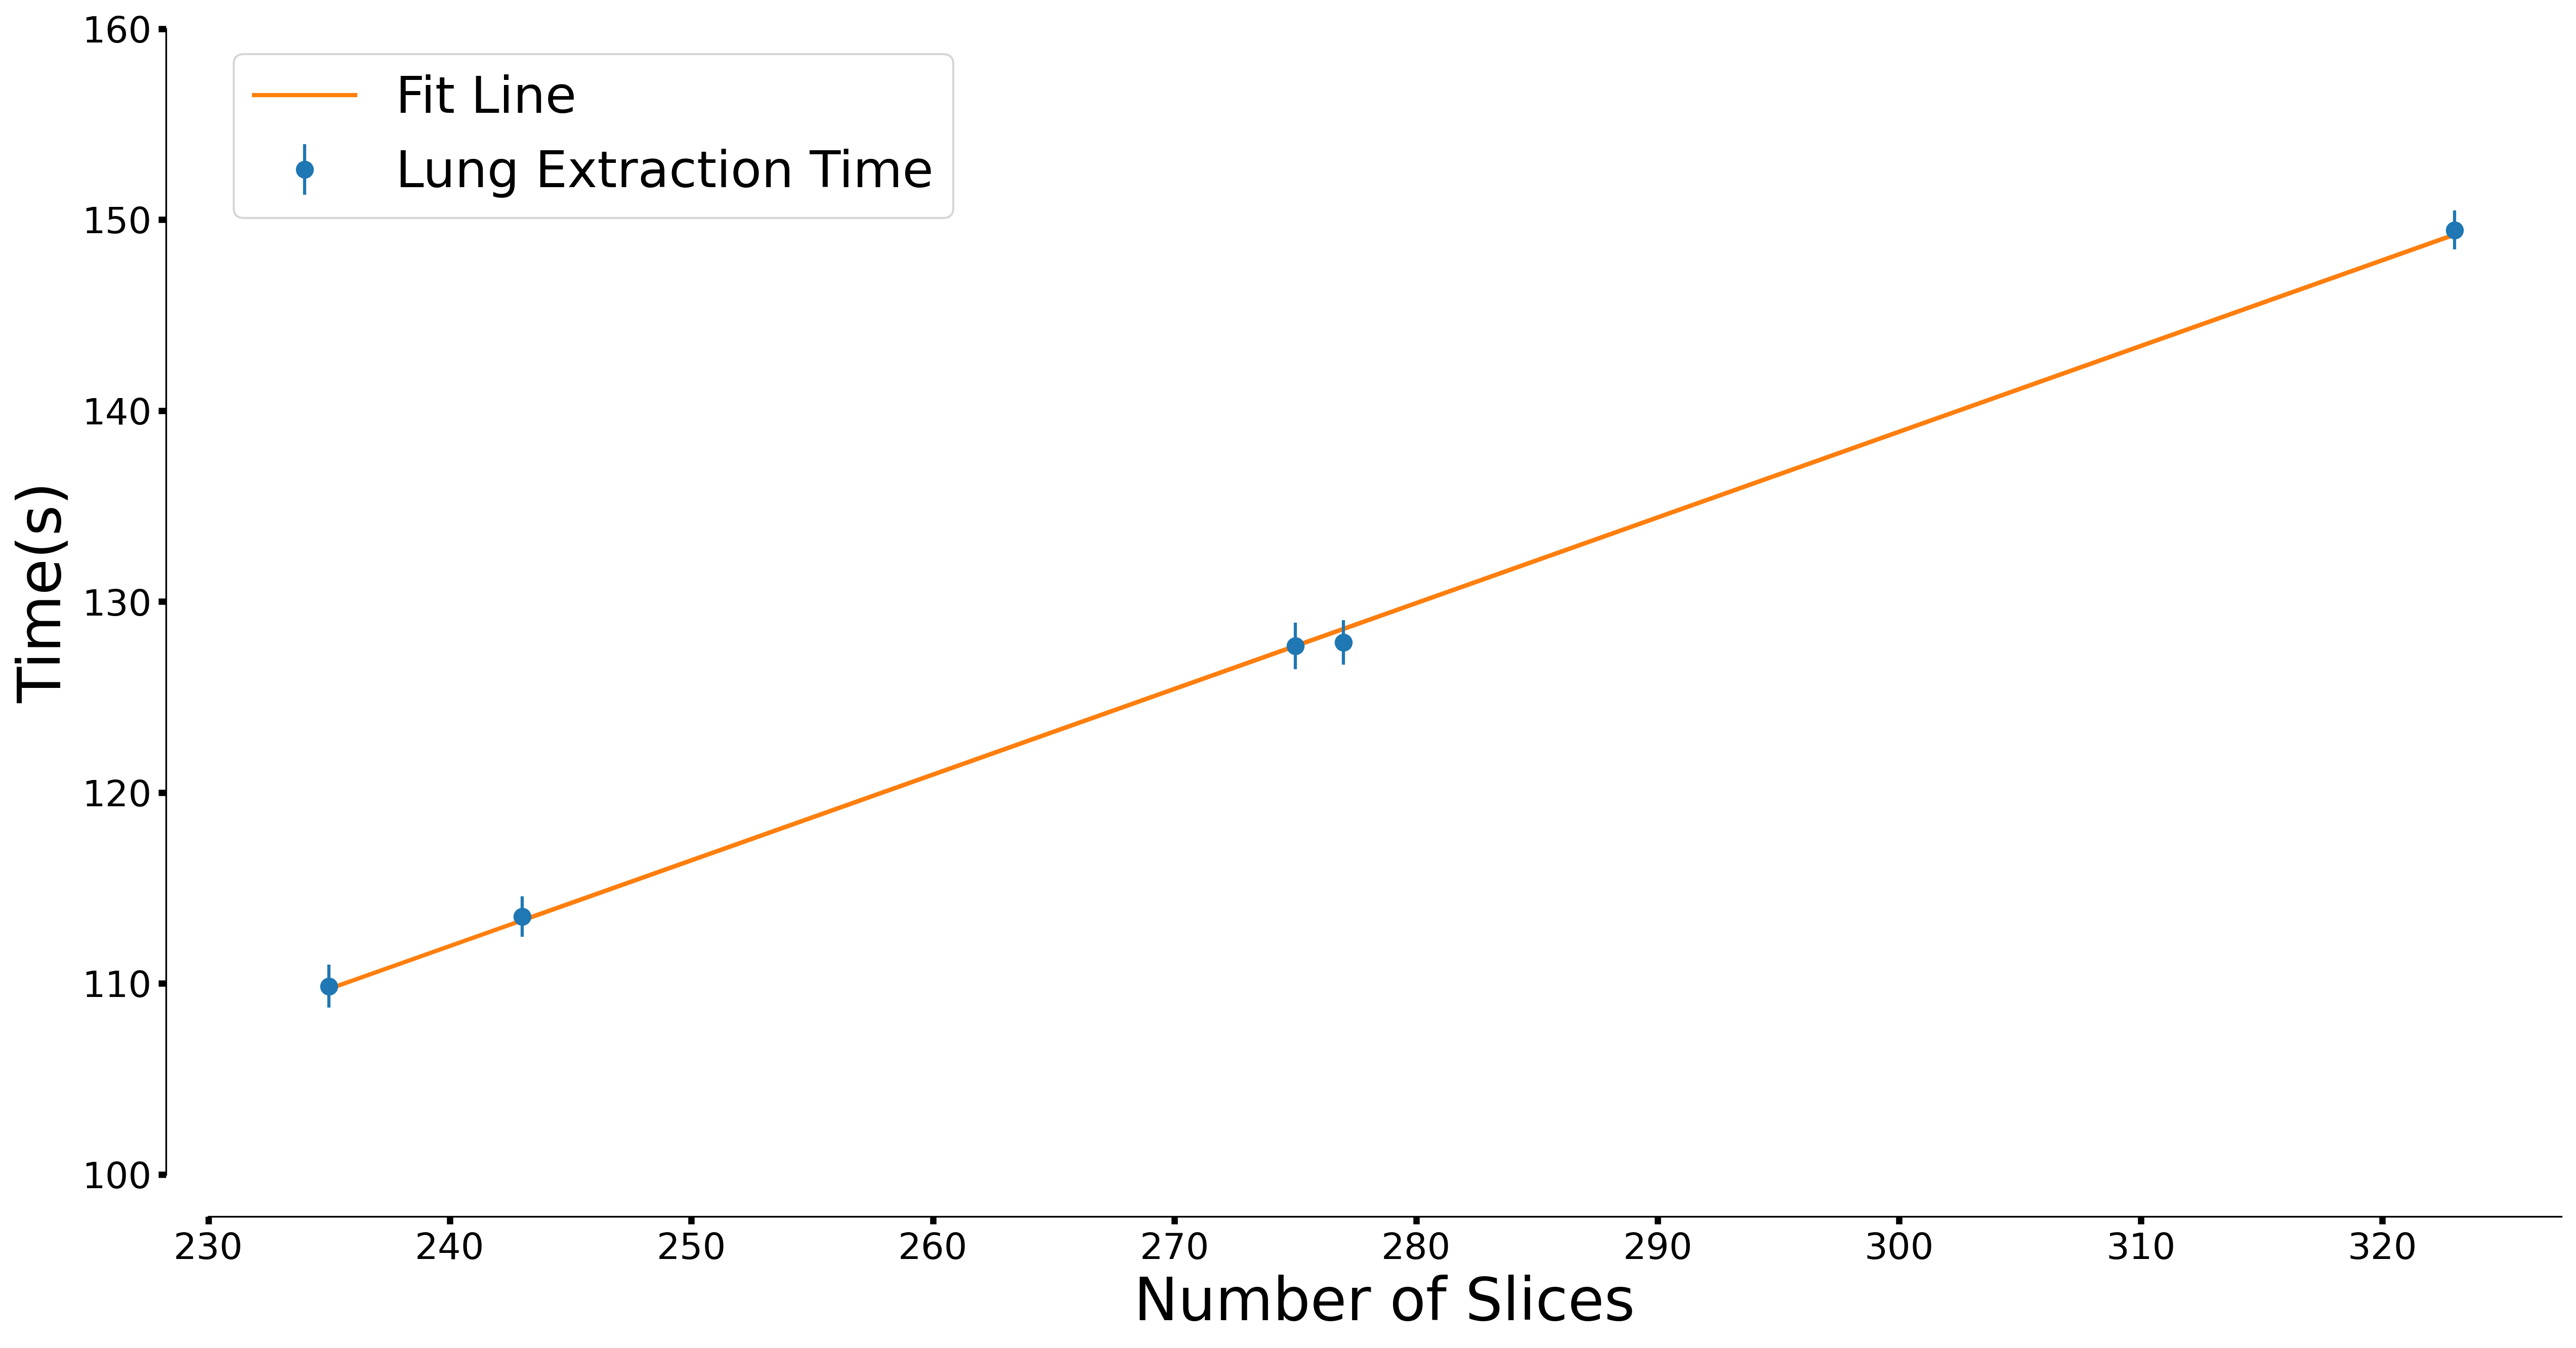
\includegraphics[width=.9\linewidth]{./img/Lung_timing}
				\centering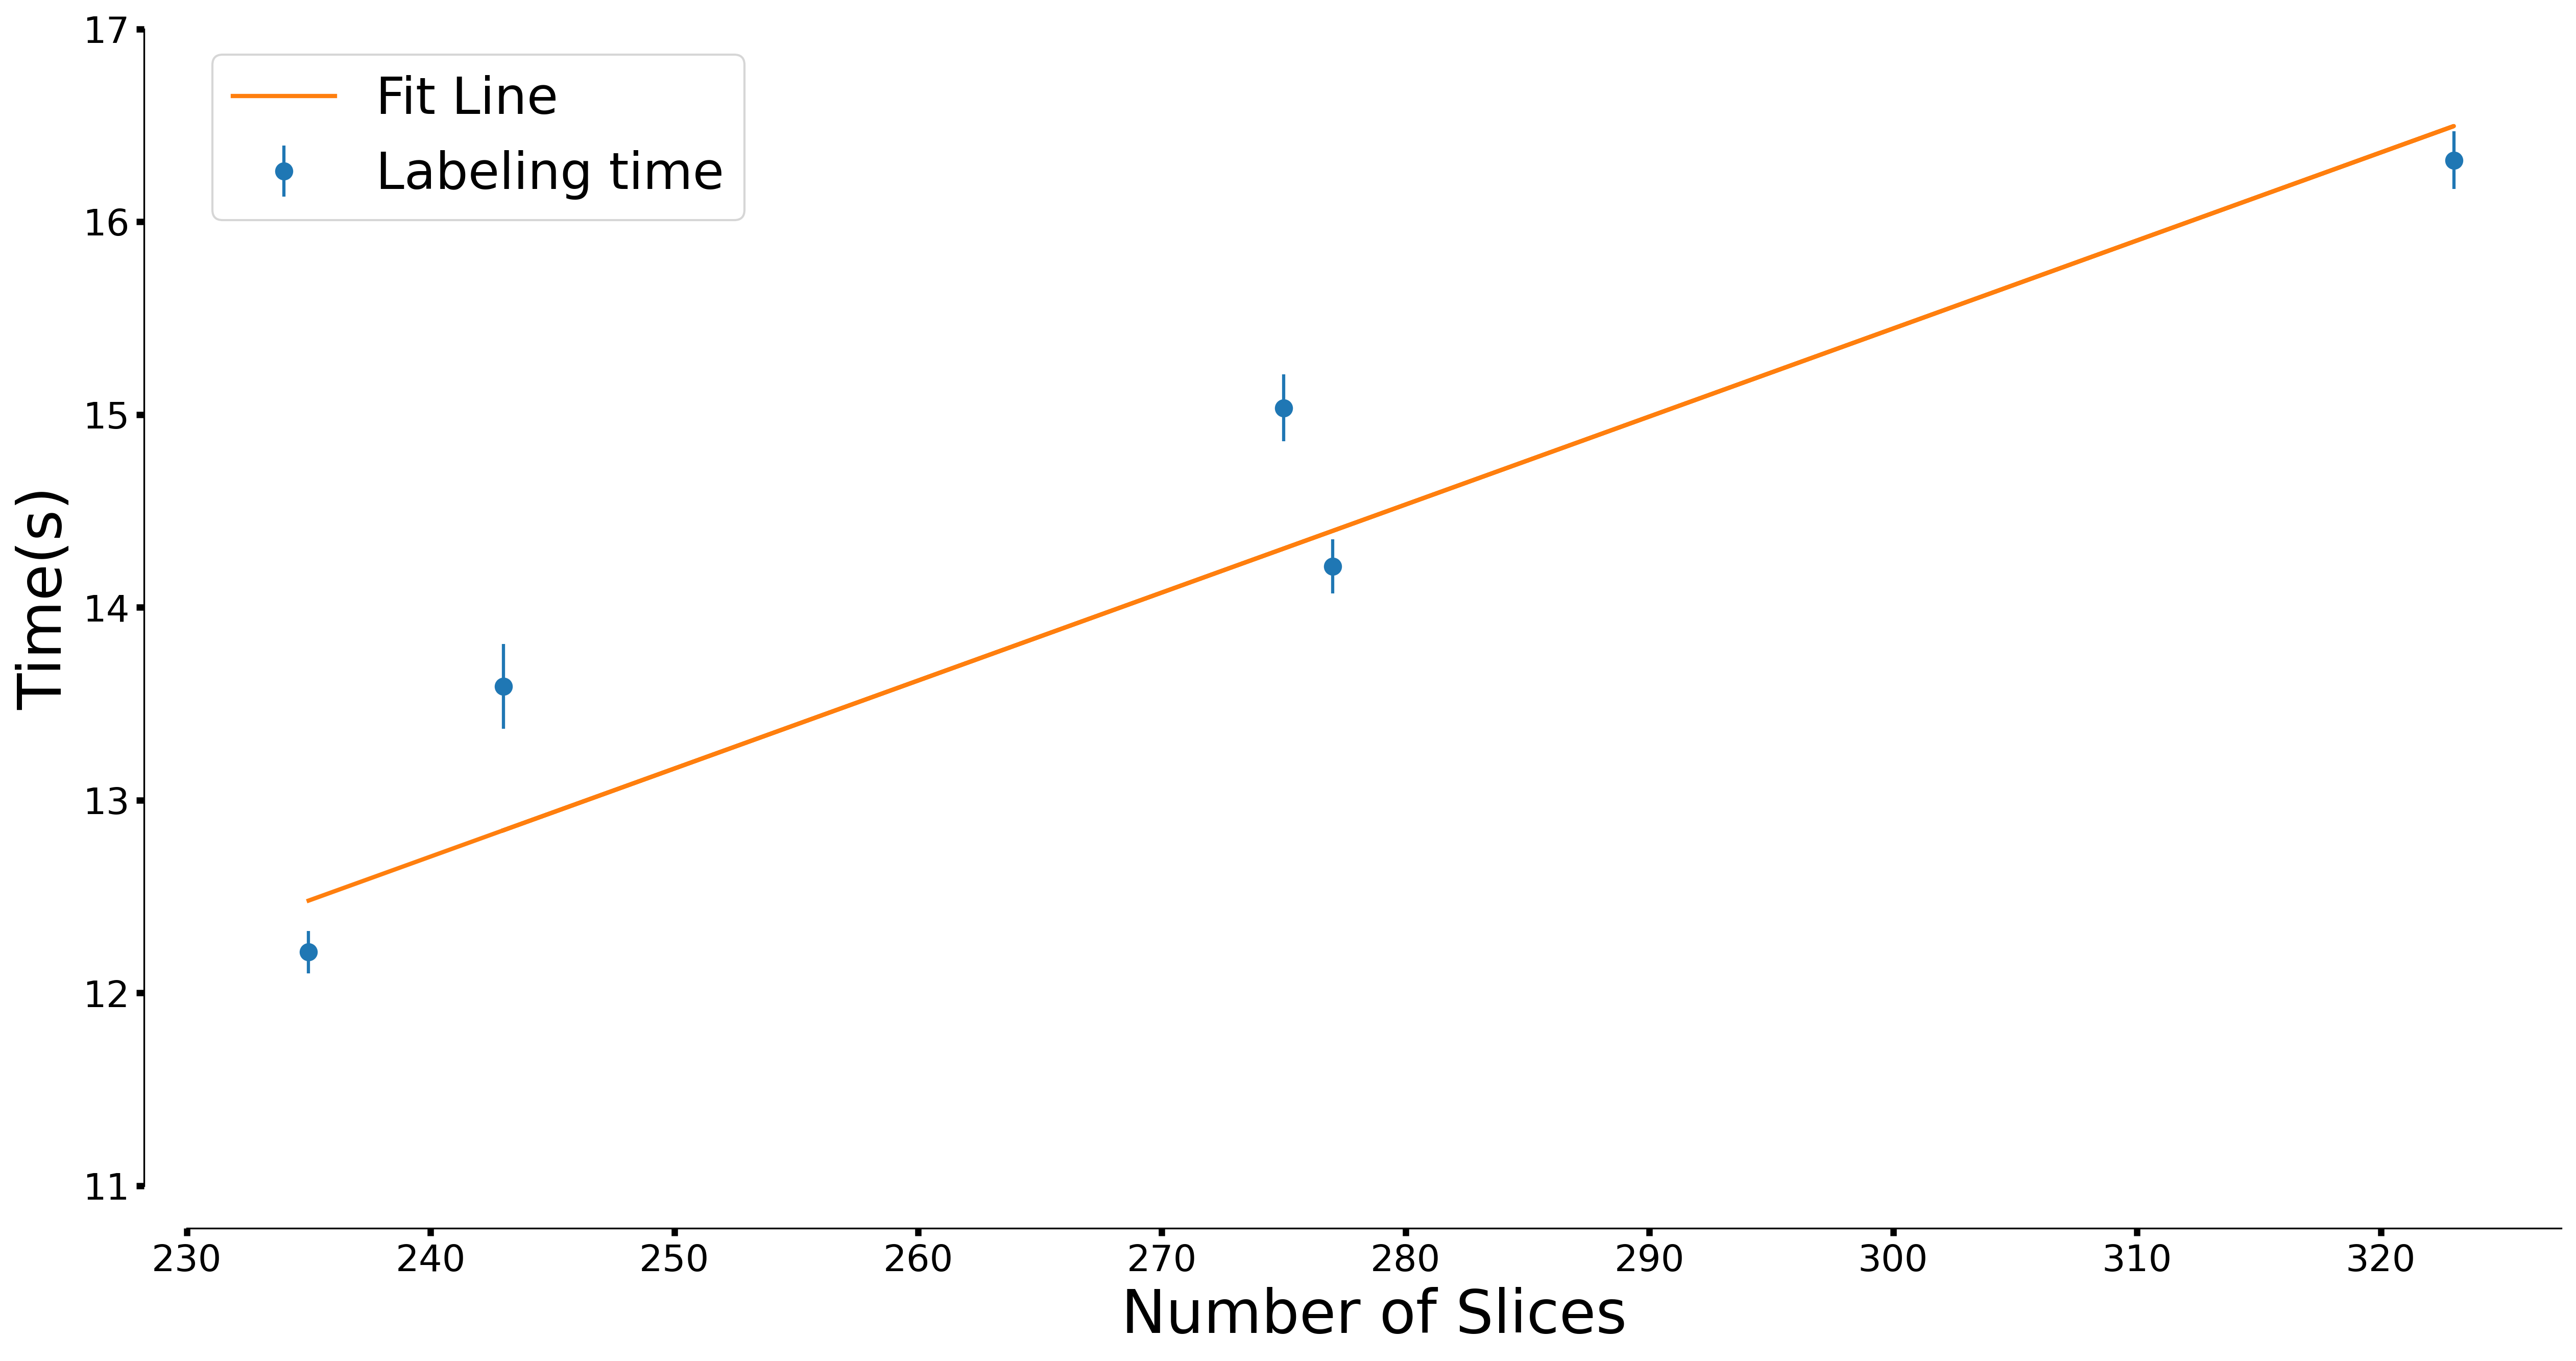
\includegraphics[width=.9\linewidth]{./img/Labels_timing}
			\end{column}
			\begin{column}{.3\textwidth}
				\begin{block}{Time per slice}
					\begin{itemize}
						\item \scriptsize\textbf{Lung Extraction:}$449.94\pm 0.03\,ms$
						\item \scriptsize\textbf{Labelling:}$45.65\pm 0.05\,ms$
					\end{itemize}
				\end{block}
			\end{column}
		\end{columns}
	\end{frame}
\end{document}